% !TeX root = ../main.tex
% Add the above to each chapter to make compiling the PDF easier in some editors.

\chapter{Dataset}\label{chapter:dataset}

The goal of this thesis is to provide a framework for compressed sensing, leveragin the strengths of deep generative models.
Methods such as by Bora et al \parencite{CSUsingAI} show very good reconstructions with fewer measurements compared to classical compresses sensing approaches.
Thus, this thesis aims at reconstructions which are highly ill-posed by having a lot of unknowns.
For this, datasets of high spatial resolution inventories are required.
To increase the number of unknowns, this thesis aims at sector-wise reconstructions, i.e. reconstructions of each sector, such as heating sector, individually.
Datasets such as CAMS \parencite{CAMS} or TNO \parencite{TNO_LowRes}  provide GHG emissions in a 0.1 times 0.05 lat times long resolution which corresponds to ~5 by ~5 kilometers.
This resolution is very low.
For instance, a city contained within a 30km by 30km grid, would contain 6 by 6 cells.
With 15 sectors, the number of unknown would be 540 for which deep learning does not make much sense as enough measurements can be made to reconstruct this perfectly using sparse reconstruction.
Therefore, this thesis focuses on the high res $2015$ \parencite{TNO_HighRes15} and $2018$ \parencite{TNO_HighRes18} TNO datasets are used.
These are two high resolution, roughly 1km by 1km, emission inventory and thus high resolution emission fields in urban environments can be extracted.
The inventory contains GHG emissions for each GNFR sector \parencite{GNFR_Sectors}, with the road sector $F$ being split into $4$ sub sectors, for each coordinate in a defined grid within Europe.
This results in $15$ emission values per gas per cell.
For this thesis, only CO2 from fossil fuels are considered.
However, the presented approaches can be directly applied for all types of GHG sources.

\section{Urban Emission Fields}
Urban environments differ from non-urban environments in terms of their emissions.
For instance, urban environments often have a city center that generates a large portion of emissions as seen for example in Munich (Figure).
\begin{figure}[h!]
    \centering
    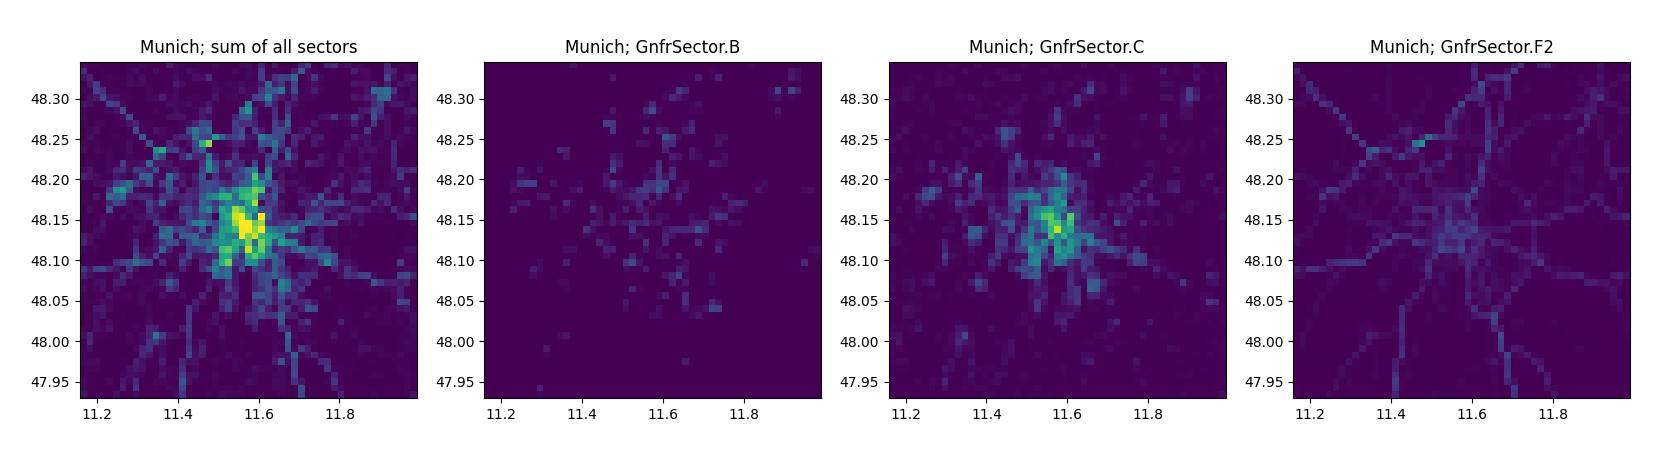
\includegraphics[width=\textwidth]{figures/03_dataset/Munich_plot.png}
    \caption{Munich Emissions}
\end{figure}
Therefore, as the focus of this thesis are urban environments, they have to be filtered from the TNO datasets.
For this, several cities are selected from a public database by OpenDatasoft \parencite{OpenDataSoft}.
Cities are filtered according to their population size.
For this thesis, the population threshold is set to $100.000$.

From the filtered cities, the coordinates are used to extract emission fields.
From the TNO dataset, $51$ by $51$ grids around the city center are extracted.
This corresponds to a dimension of n km by n km.
While most cities are not even close to this size, this allows to later crop the fields to a desired size.
For this thesis, emission fields have $32$ by $32$.

Some cities may be too close to each other and thus result in leakage of data to test and validation sets.
Thus, cities are filtered if they are too close to other cities.
The following algorithm is used to guarantee no overlapping data.
1) Get all cities currently extracted and determine the lat and lon distances to the current city
2) Determine all cities that are within a threshold
3) If there are none, add the current city and proceed to next city
4) Else, check if the current city has a greater population size that all other cities that overlap
5) If yes, removed the overlaping cities and add the current city to the cities.
6) Else, ignore the city and proceed with next city

The overall resulting amount of city emission fields per year, $2015$ and $2018$, is then $106$.
However, Bratislava has been identified as an outlier for this dataset.
Therefore, Bratislava is removed and the number of cities is reduced to $105$.
(Add method of how Bratislava was detected as outlier)
A list of all cities with the corresponding coordinates is appended in the appendix.

The number of extracted emission fields is not enough to train a generative model.
Thus, temporal scaling factors from \parencite{ScalingFactors} are used to generate more samples.
Scaling factors are applied to individual GNFR sectors.
This results in $24 * 7 * 12 = 2016$ samples per city per year.
The resulting combined dataset size is then $106 * 2 * 2016 = 45792$ individual emission fields with size $51$ by $51$.
To reduce the memory overhead, scaling factors are applied at sampling time and only the original data is kept in memory.

\section{Dataset Split}
The emission fields are split into training, validation, and test data.
The test data is used for experiments and evaluations and makes up $t$ percent of the data.
The model does not see the test data during training.
The validation data is used to evaluate the generalization capabilities of the model during training and makes up $v$ percent of data.
Finally, the training data is used to train the model and updates its weights and makes up $1 - v - t$ of the data.

Emissions of cities may vary in terms of their mean emissions.
Splitting the dataset randomly may result in splits that are not representative of each other.
For instance, a higher mean emission per city in the validation data results in a higher MSE in the validation step as the MSE is sensitive to scale.
Thus, an appropriate split of data shall distribute cities equally in terms of their mean emissions.
In other words, validation, test, and trianing data shall have the same distribution of city sizes to assess generalization abilities the best. 
Furthermore, individual cities shall not leak into the other datasets.
For instance, data from 2015 of Berlin shall not end up in the test set while 2018 data ends up in the train data.
To achieve a split that satisfies both requirements and is reproducible, the following algorithm is used:
First, fields are grouped according to their city names.
Then, the city names are sorted according to their mean emissions in descending order.
Afterwards, the test data is determined, by computing \dots (missing explanation of algorithm here)

First, $t$ percent of the data is assigned to the test data using this algorithm.
Then, of the remaining $1 - t$ percent of data, $\frac{v}{1 - t}$ of data is assigned to the validation data.
The remaining data is then assigned to the training set.

Maybe make a diagram here.

\section{Data Augmentation}
To improve the generalization abilities of the model CITE, common image augmentation techniques are applied (to cite) to the emission fields in the training data.
First, random cropping is used.
Furthermore, a random horizontal flip and vertical flip are applied with probability $0.5$ each.
Lastly, emission fields are randomly rotated by 90$\circ$ with probability of $0.5$.
This results in $8$ different transformations, with one of them being the original emission field.
\begin{figure}[h!]
    \centering
    \includegraphics[width=\textwidth]{figures/03_dataset/nürnberg_city_plot.png}
    \caption{Example Training Sample}
\end{figure}

The validation and test emission fields are not transformed, except for a center crop to the expected dimensions.

\section{Scaling}
Scaling is an important factor for machine learning.
Large-scale data can make training converge slow and instable (cite).
Furthermore, regularization techniques such as batch normalization \parencite{BatchNorm} rely on scaled values (cite).
A common technique for scaling values is min max scaling (cite).
However, min max scaling is sensitive to outliers and thus not ideal for emission inventories where range of emissions within a city can largely differ.
Instead, robust scaling (cite) can be applied.
To determine a good scaling factor, the $95$th percentile of values is determined for each city in the training set.
The inverse of the average is then used as the scaling factor.
The resulting scaling factor is thus $\frac{1 a}{2.5 * 10^6 kg}$ after rounding.

All experiments are, without loss of generality, performed on the scaled data.

\section{Case Studies}
Besides the test data for evaluating the performance of the model, three cities are chosen for case studies.
The cities are: Munich, Zurich, and Paris.
These cities are chosen in accordance to the Icos project \parencite{Icos} and represent three different sizes, i.e. smaller, medium sized, and large, well.
These cities are removed from the dataset before splitting, reducing the overall amount of available cities for training to $102$.

These cities allow closer inspection of the outputs of different algorithms
